\subsection{Mapeamento 3D}

Muitos dos problemas encontrados na operação de inserção e remoção dos
\textit{stoplogs} são provenientes da existência de objetos estranhos, trazidos
pelo próprio rio, presentes no leito de concreto ou na superfície de um dos
\textit{stoplogs}. A inspeção da existência de tais objetos, isto é, a sua
visualização, é de suma importância para que se possa determinar corretamente
qual ação corretiva é a mais apropriada.

Em ambientes subaquáticos onde o meio possui uma boa visibilidade, é possível a
utilização de câmeras para a realização da inspeção. Porém em ambientes onde a
visibilidade não é satisfatória, a utilização de câmeras fica inviabilizada.
Para esses casos, é necessário a utilização de Sonares para a
visualização do ambiente a ser inspecionado. Porém os Sonares utilizados para
mapear os ambientes não tem uma resposta que é facilmente interpretada pelo ser
humano e, por isso, é necessário que se faça uma conversão dos dados e uma a
construção de uma representação 3D da superfície.

Nesta secção será apresentado o que é o sensor Sonar e determinando através de uma análise técnica e de fornecedores qual o Sonar que atende aos requisitos de projeto. Assim como, será descrito qual tecnologia de mapeamento 3D será aplicada ao projeto. 



\subsubsection{Sonar}
Sonar\footnote{A sigla tem origem como acrônimo de \textit{sound navigation and ranging}.} é uma técnica que utiliza a propagação do som na água para se comunicar e detectar objetos nesse meio, ela possui duas vertentes uma chamada ativa e outra passiva. A passiva se resume a escutar o meio e não será investigada, pois não possui a funcionalidade para o mapeamento de superfícies submersas. Os equipamentos que fazem uso de tal tecnologia acabam por herdar seu nome, assim sonares que utilizam a tecnologia ativa são chamados de sonares ativos.

O sonar ativo, daqui em diante apenas referido como sonar, emite um ping que é um pulso de onda sonora que será refletido pelo meio. Conforme a frente de onda atravessa os objetos submersos ela é refletida e este eco é detectado no retorno pelo sonar, onde ele extrai as informações do tempo que a onda levou para retornar e sua intensidade, podendo, a partir do conhecimento de características do meio, como a velocidade de propagação do som, estimar a distancia de origem do eco e consequentemente do objeto.

Pela aplicação os sonares são divididos em basicamente duas categorias: \emph{profiling} e \emph{imaging};

O sonar do tipo \emph{imaging} são tipicamente utilizados para fazer o mapeamento do fundo do mar, possuindo uma abertura em formato de leque (ver figura~\ref{sonar_1}), eles podem utilizar um motor de rotação sobre o eixo perpendicular ao feixe ou podem ser arrastados pela água para fazer o escaneamento (ver figura~\ref{sonar_2}).

\begin{figure}[H]
    \centering
    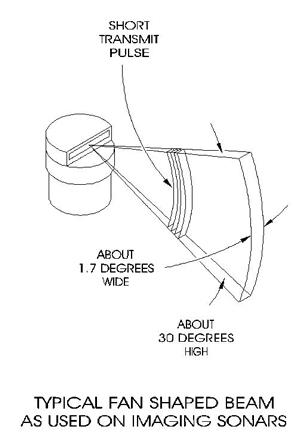
\includegraphics[width=0.5\columnwidth]{figs/sonar/1.jpg}
    \caption{Típico feixe em formato de leque de sonares tipo \emph{imaging}}
    \label{sonar_1}
\end{figure}

\begin{figure}[H]
    \centering
    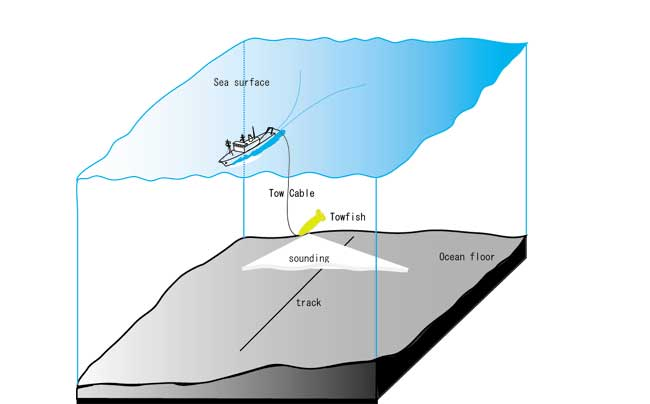
\includegraphics[width=0.5\columnwidth]{figs/sonar/2.jpg}
    \caption{Sonar \emph{imaging} sendo arrastado para mapeamento das profundezas}
    \label{sonar_2}
\end{figure}


A resposta dos sonares tipo \emph{imaging} forma uma imagem colorida exibindo tons diferentes para respostas mais fortes e mais fracas de eco do sonar. Sendo utilizado para obter uma imagem do fundo do mar semelhante as que os radares fazem na superfície.

Pela tecnologia empregada os sonares \emph{imaging} possuem dois tipos de configuração: \emph{multibeam} e \emph{mechanical} (single beam).

A configuração \emph{single beam} possui um transdutor acoplado a um mecanismo de \emph{pan} para possibilitar a varredura de determinada área. Assim, o sonar envia seu \emph{ping} espera o eco de retorno e avança para a próxima posição determinada pelo passo, ou resolução angular, do motor que compõe o mecanismo de \emph{pan}.

Alternativamente, os sonares \emph{multibeam} possuem idealmente um feixe \emph{ping} extremamente amplo, sendo na prática composto por diversos feixes com seus respectivos transdutores sincronizados. Essa configuração possui diversos receptores espalhados por uma região do sonar, resolvendo qual a posição de origem do eco através de um sistema de multilateração. Assim, o \emph{multibeam} sobrepuja a configuração \emph{single beam} no aspecto de precisão e tempo de varredura.

De forma diferente, os sonares do tipo \emph{profiling} retornam apenas um valor e não uma graduação de tons. Esse valor é referente, normalmente, ao tempo de retorno do eco mais intenso dentro do intervalo de amostragem, intervalo de espera que delimita o alcance máximo de interesse. Esses sonares também podem ser configurados para enviarem o valor do tempo de retorno do primeiro eco, em vez do mais intenso, de maneira a agilizar o processo de captura de dados, pois todos os ecos à partir do primeiro são ignorados, passando para a emissão de um novo \emph{ping} em uma nova posição.

Outra característica importante dos sonares \emph{profiling} é o formato do seu feixe, este possui uma abertura estreita de formato tipicamente cônico (ver figura~\ref{sonar_3}).

\begin{figure}[H]
    \centering
    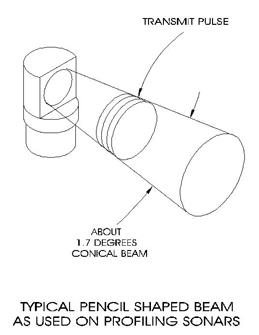
\includegraphics[width=0.5\columnwidth]{figs/sonar/3.jpg}
    \caption{Típico feixe em formato de cone de sonares tipo \emph{profiling}}
    \label{sonar_3}
\end{figure}

A figura \ref{sonar_4}) demonstra comparativamente a diferença entre os diferentes tipos de sonares.

\begin{figure}[H]
    \centering
    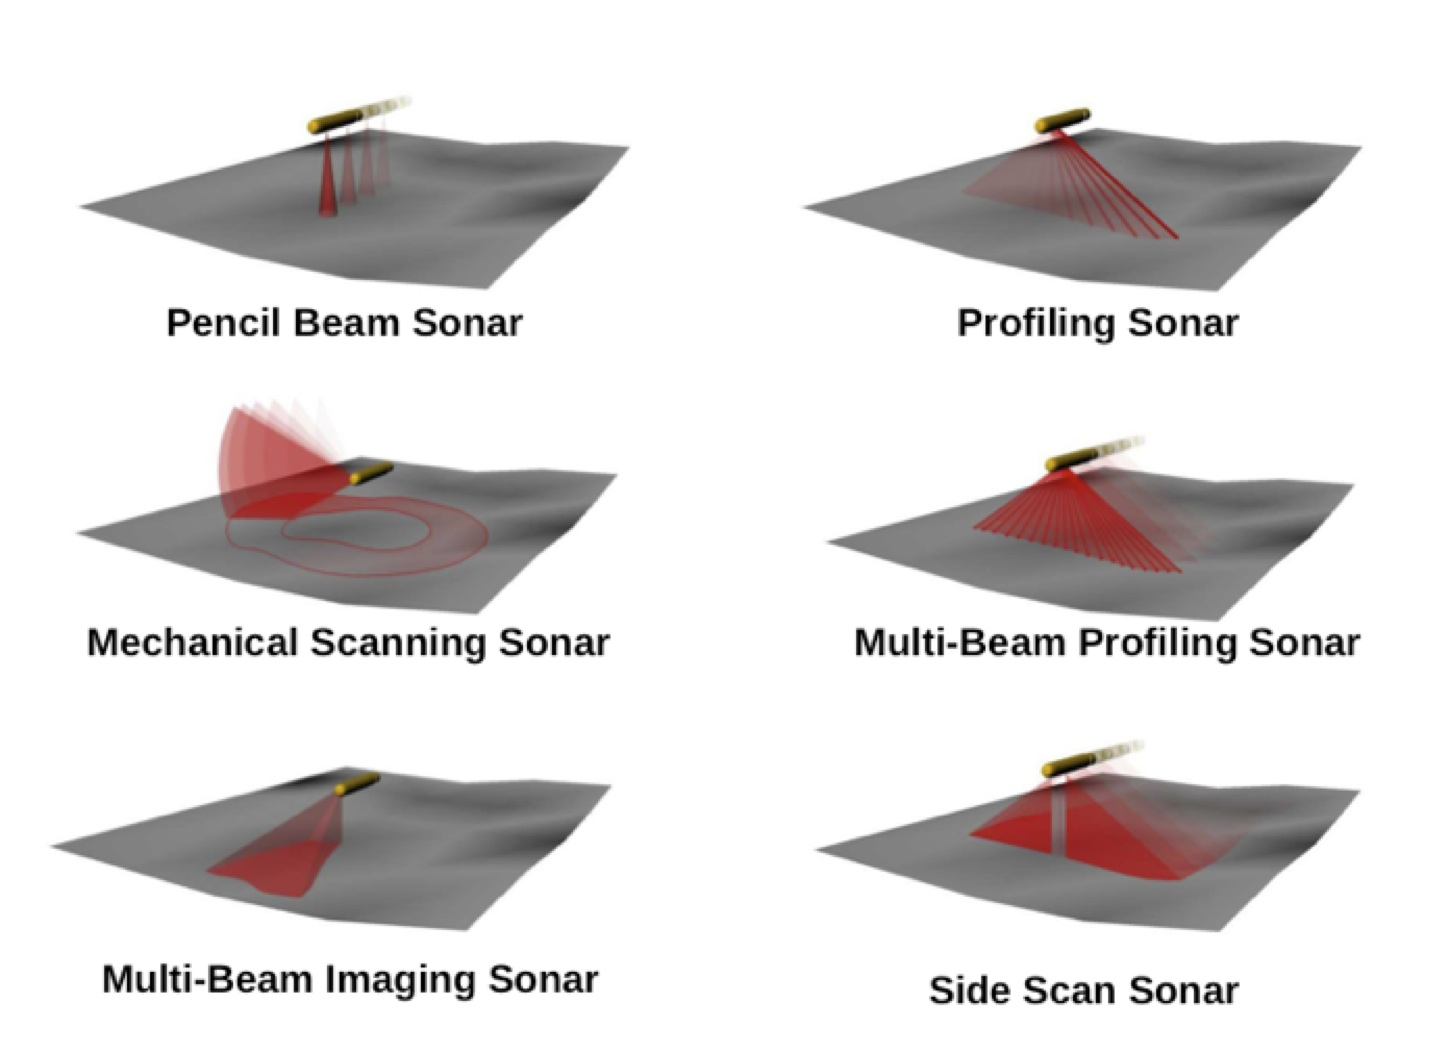
\includegraphics[width=1\columnwidth]{figs/sonar/4.jpg}
    \caption{Tipos de Sonares}
    \label{sonar_4}
\end{figure}


 \paragraph{Conclusão de análise técnica}\mbox{}\\
 O ambiente no qual será utilizado o sonar possui uma profundidade inferior a 20
 metros e a necessidade de mapeamento se localiza sobretudo em uma área de
 aproximadamente $2 \times 15 m^2$. Para essa situação o sonar profiling se
 mostra como o mais apropriado devido ao seu estreito feixe que otimiza a
 precisão para uma pequena superfície pouco profunda. 

Os fornecedores e modelos pesquisados estão apresentados na tabela abaixo. Dentre os modelos análisados o Super Seaking DFP e Micron apresentam o melhor custo. A diferença de custo entre ambos os modelos se dá devido a diferença da abertura do feixe. O Super Seaking DFP possui um feixe mais estreito, o que permite uma maior precisão. Não é possível determinar qual seria o modelo mais aplicável apenas por análise teória, logo parte da pesquisa deste projeto será testar ambos os modelos para determinar qual é o mais aplicável.  


\begin{center}
    \begin{tabular}{| l | l | l | l | }
    \hline
	{\bf Modelo} & 	{\bf Fabricante} &		{\bf Distribuidor}	&	{\bf Preço} \\  \hline
	BV5000 &			Blueview&				- &					323.000,40R{\$} \\  \hline
	3D Echoscope&	Octopus&		 		Seatronics&			960.000,00 R{\$} \\  \hline
	DT101&			Imagenex&			Marine Solution&	365.000R{\$} \\  \hline
	Super Seaking DFP&		Tritech&				MacSea&			33.990,50R{\$} \\ \hline
	Micron Sonarg &		Tritech&				MacSea&			16.798,90R{\$} \\ \hline

\hline 
\end{tabular}
\end{center}


\subsubsection{Unidade Pan e Tilt}

O sonar tipo profiling definido possui apenas 1 grau de liberade interno, logo não é possível mapear toda a região do trilho do stoplog com o mesmo a partir de uma posição fixa de acoplamento na garra pesacdora. Logo, uma unidade de pan e tilt será acoplado ao Sonar possibilitando assim cobrir toda a extensão do trilho do Stoplog. 

O fator mais importante na escolha do motor de posicionamento é a precisão que o mesmo consegue operar, pois o sonar mede a distância ao meio que se encontra de 3 a 50 metros de distância do mesmo, logo um pequeno erro de posicionamento angular do motor resultará em um erro grande na reconstrução do meio. Exemplo: 1 grau de erro a 50m de distância significaria 0,87m de erro na reconstrução do ambiente. A tabela abaixo lista alguns dos modelos disponíveis no mercado, sua precisão dada a folga mecânica do mesmo e o custo.  Logo, o modelo escolhido para o projeto foi o OE10-102 da Kongsberg que oferece a menor folga mecânica.

\begin{center}
    \begin{tabular}{| l | l | l | l | }
    \hline
	{\bf Modelo} & 	{\bf Fabricante} &		{\bf Folga}	&	{\bf Preço} \\  \hline
	PT-10FB &			ROS&				0.6deg &		24.101,90 R{\$} \\  \hline
	SS109&				Sidus&				 0.5deg&			14.576,57 R{\$} \\  \hline
	OE10-102&			Kongsberg&			0.08 def&	 		29.441,40 R{\$} \\  \hline

\hline 
\end{tabular}
\end{center}

%%%%%%%%%%%%%%%%%%%%%%%%%%%%%%%%%%%%%%%%%%%%%%%%%%%%%%%%%%%%%%%%%%%%%%%%%%

\subsection{Reconstrução de superfície 3D}

Uma reconstrução 3D de superfície consiste na interpretação e combinação de
dados, afim de se extrair informações tridimensionais do ambiente. Em ambientes
subaquáticos com pouca visibilidade, o sensor recomendado para esse tipo de
operação é o sonar. A figura \ref{figs/3d/3dcomporta} exemplifica uma
reconstrução 3D obtida pelo processamento de dados provenientes de um sonar.
\begin{figure}[H]
    \centering 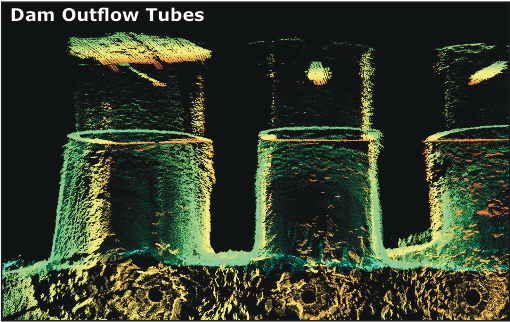
\includegraphics[width=0.9\textwidth]{figs/3d/3dcomporta}
    \caption{Exemplo de uma reconstrução 3D da sáida de uma barragem dos dados obtidos de um sonar 3D.}
    \label{figs/3d/3dcomporta}
\end{figure}


Um dos pontos determinantes para uma boa reconstrução 3D é a forma de se representar e armazenar as informações tridimensionais, já interpretadas dos sensores. Uma boa representação 3D deve possuir uma boa fidelidade do ambiente real representado, ter boa velocidade de processamento e pouca utilização de memória do sistema.

Após a revisão bibliográfica realizada, os tipos de armazenamento e representação mais recentes e avançados existentes na literatura eram a representação a partir de pointclouds, mapas de elevação e octomaps. A representação escolhida foi a por meio de octomaps. A seguir será realizado uma descrição das principais característica de cada método.
\begin{itemize}
    \item \textbf{Pointcloud} - Armazena as coordenadas tridimensionais de cada ponto lido pelo sensor. Possui uma boa fidelidade de representação de ambientes 3D complexos, porém não é capaz de distinguir entre espaçoes vazios e ocupados.

    Por amazenar informações ponto a ponto, não possui uma eficiente utilização de memória. A figura \ref{fig:pointcloud} mostra a representação utilizando pointcloud de uma área externa.

    \begin{figure}[H]
    \centering
    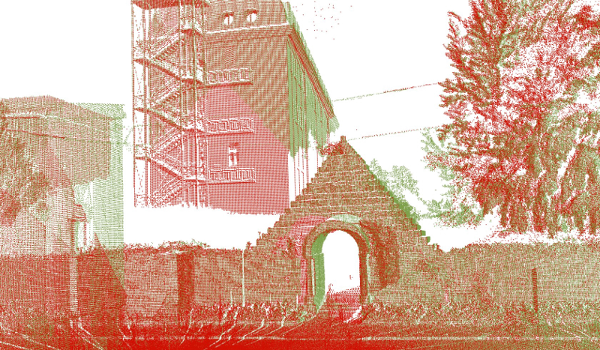
\includegraphics[width=0.8\textwidth]{figs/3d/registration_closeup}
    \caption{Exemplo de uma reconstrução tridimensional representado por uma Pointcloud}
    \label{fig:pointcloud}
\end{figure}


    \item \textbf{Mapas de elevação} - Os mapas de elevação representam uma superfície através de um grid 2D e armazenam uma informação de elevação para cada célula. Os mapas de elevação tem uma melhor eficiência de memória, porém para atingir essa virtude perdem o poder de representação fiel em todas as dimensões. A figura \ref{fig:elevacao} mostra a representação utilizando mapas de elevação de uma área externa.

    \begin{figure}[H]
    \centering
    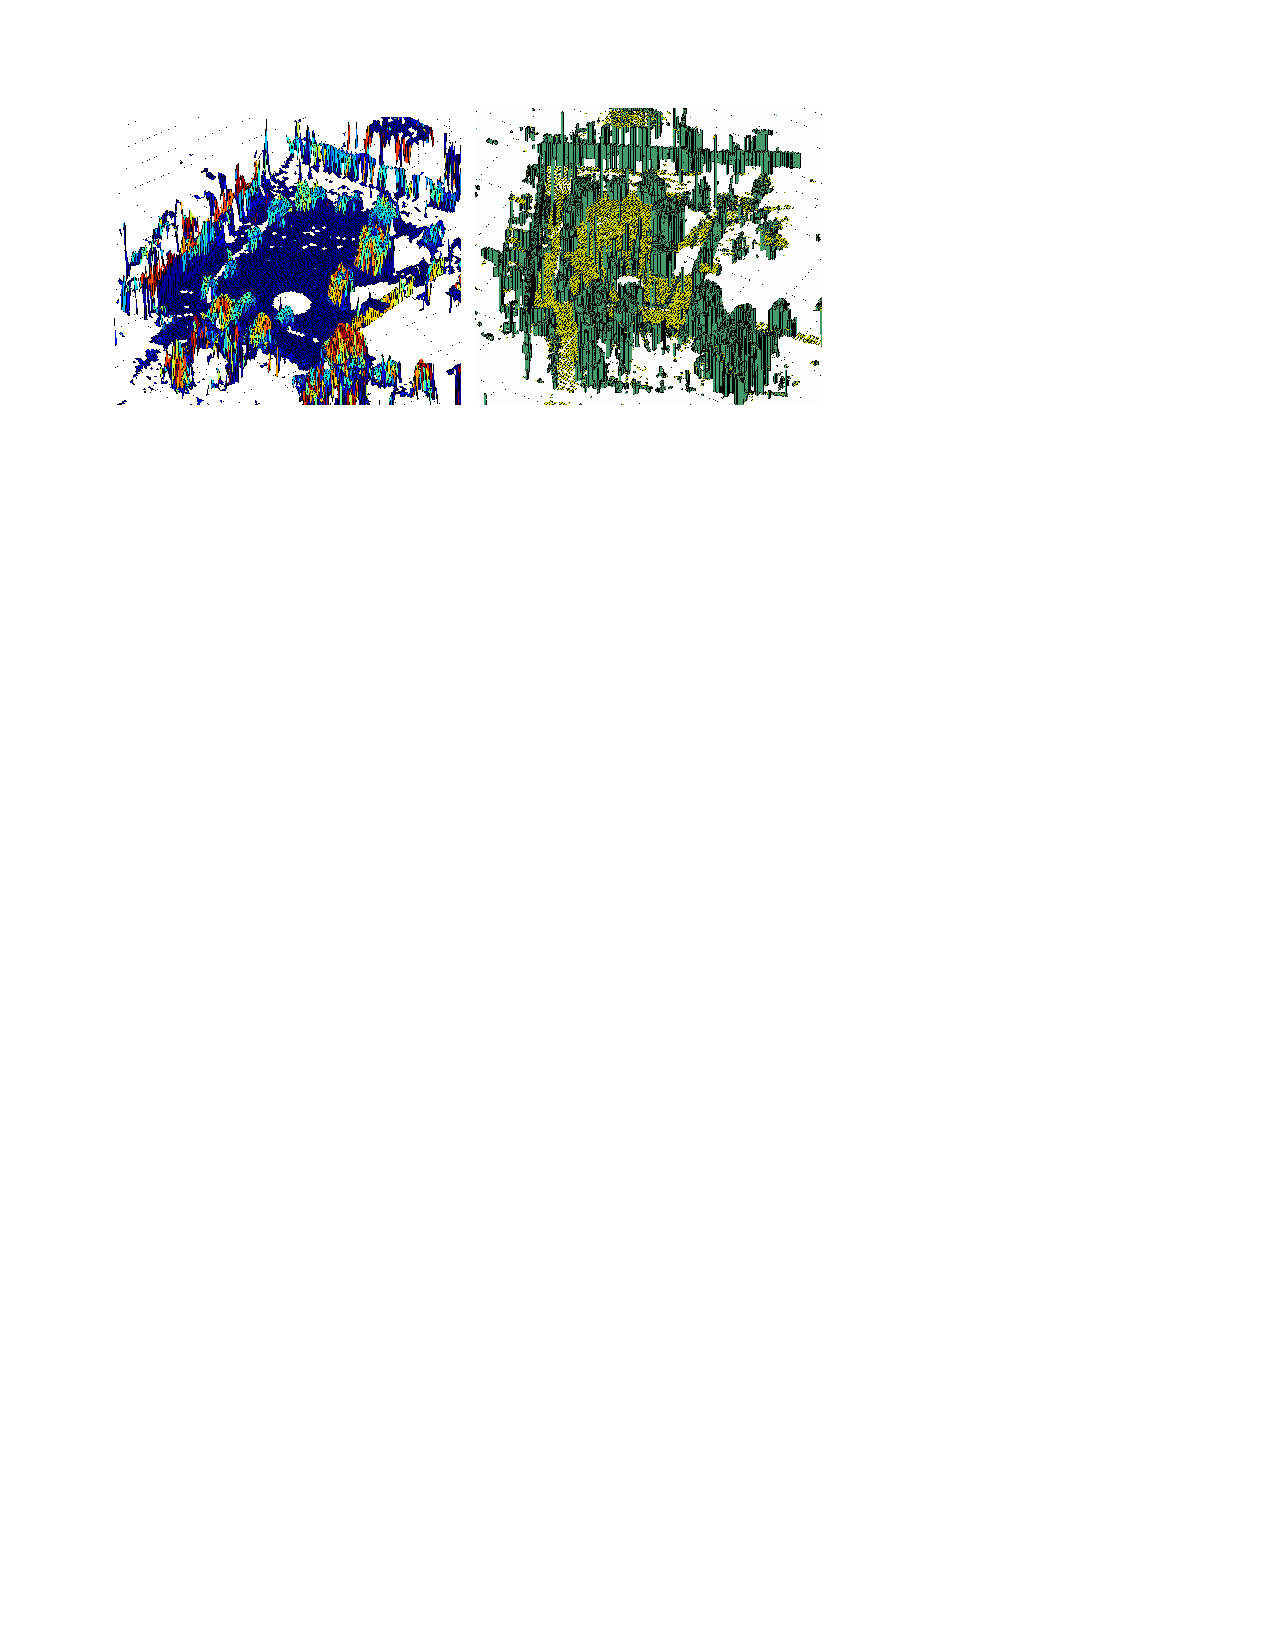
\includegraphics[width=0.8\textwidth]{figs/3d/elevationmap}
    \caption{Exemplo de uma reconstrução tridimensional representado por um Mapa de Elevação}
    \label{fig:elevacao}
\end{figure}

    \item \textbf{Octomap} - Octomap é um framework livre para mapeamento 3D baseado em uma estrutura hierárquica árvore de dados, chamada OcTree. O espaço tridimensional é recursivamente dividido em octantes, como exemplificado na figura \ref{fig:octree}. Aliada à estrutura de árvore, essa característica possibilita que somente a coordenada do ponto raiz do mapa necessite ser armazenada e todas as coordenadas dos demais pontos são inferidas através da posição relativa ao ponto raiz. Diminuindo, assim, a utilização de memória do sistema. A estrutura hierárquica possibilita, também, que no mapa gerado seja realizada buscas, segmentações para a análise separada de diferentes objetos e múltiplas resoluções, diferentemente de mapas de resolução fixa como no caso da representação com pointclouds.

    \begin{figure}[h!]
    \centering
    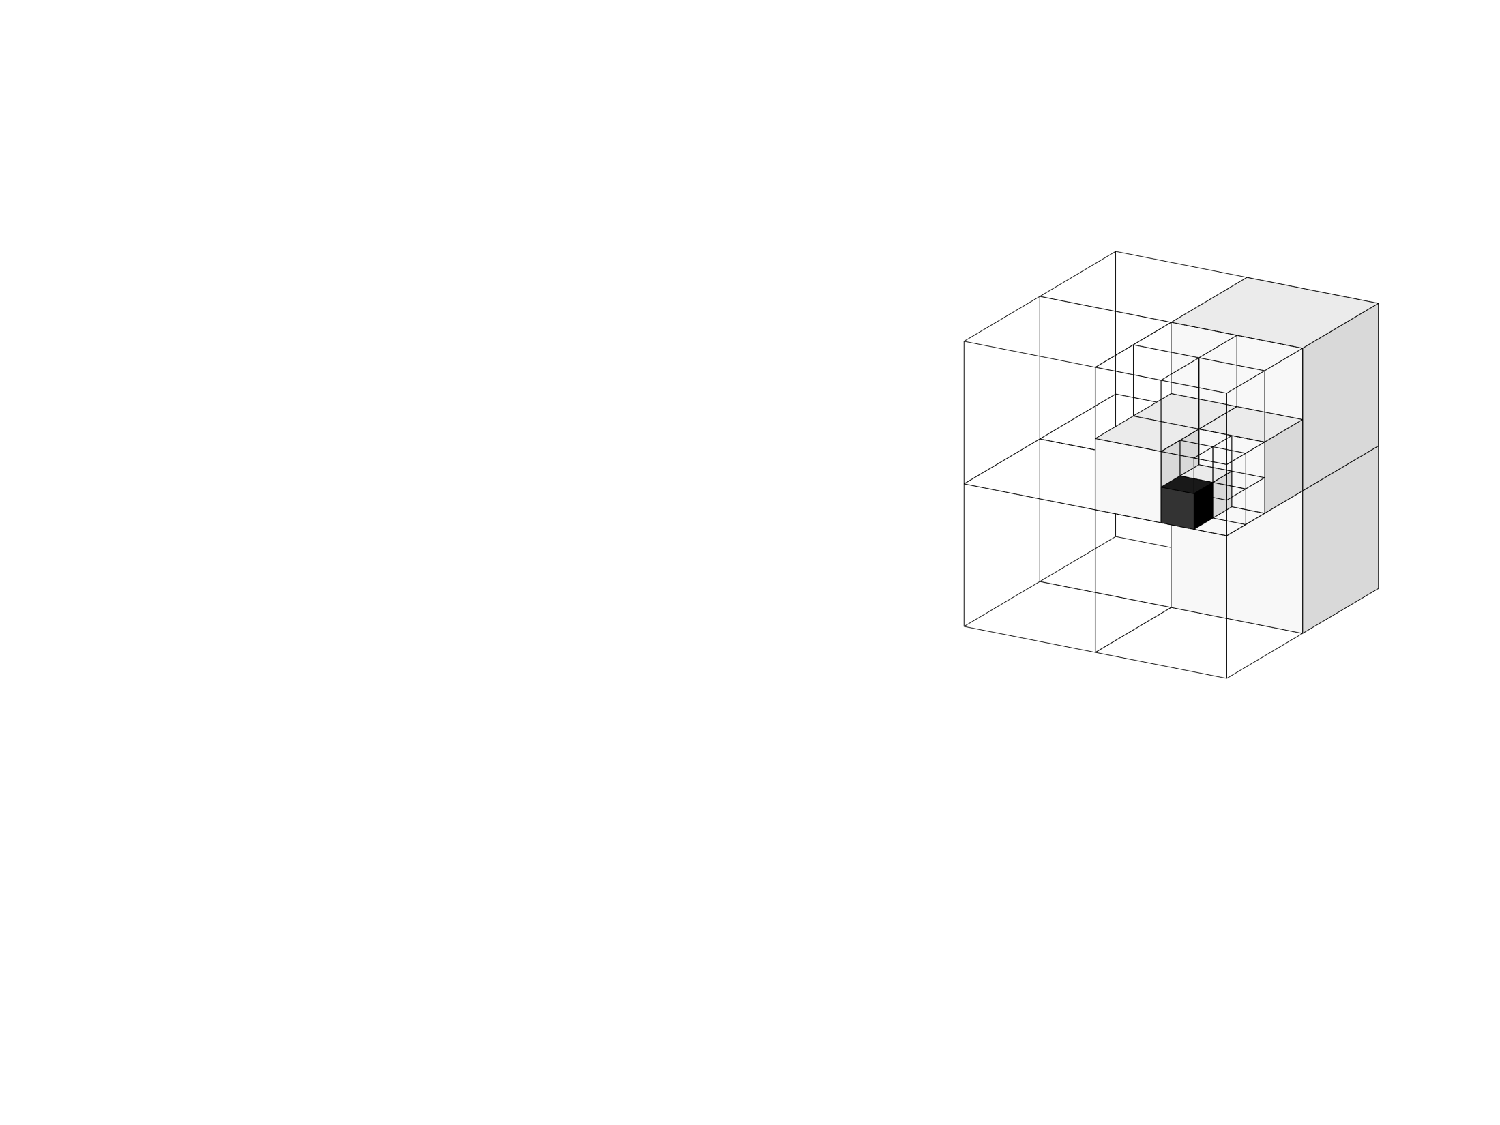
\includegraphics[width=0.4\textwidth]{figs/3d/octree}
    \caption{Divisão recursiva do espaço em octantes}
    \label{fig:octree}
\end{figure}
    O framework utiliza uma política de ocupância probabilística, o que possibilita uma boa caracterização de ambientes dinâmicos e atenuação de ruídos provenientes dos sensores. Outra vantagem importante é a diferenciação de espaços ocupados, vazios e desconhecidos, funcionalidade que não está presente em nenhum dos métodos já apresentados. A distinção entre espaços que estão desocupados e espaços ainda não explorados pelo sistema  pode ser visualizada na figura \ref{fig:free} e também uma comparação com a utilização de pointclouds para o mapeamento do mesmo ambiente.

    \begin{figure}[h!]
     \centering
    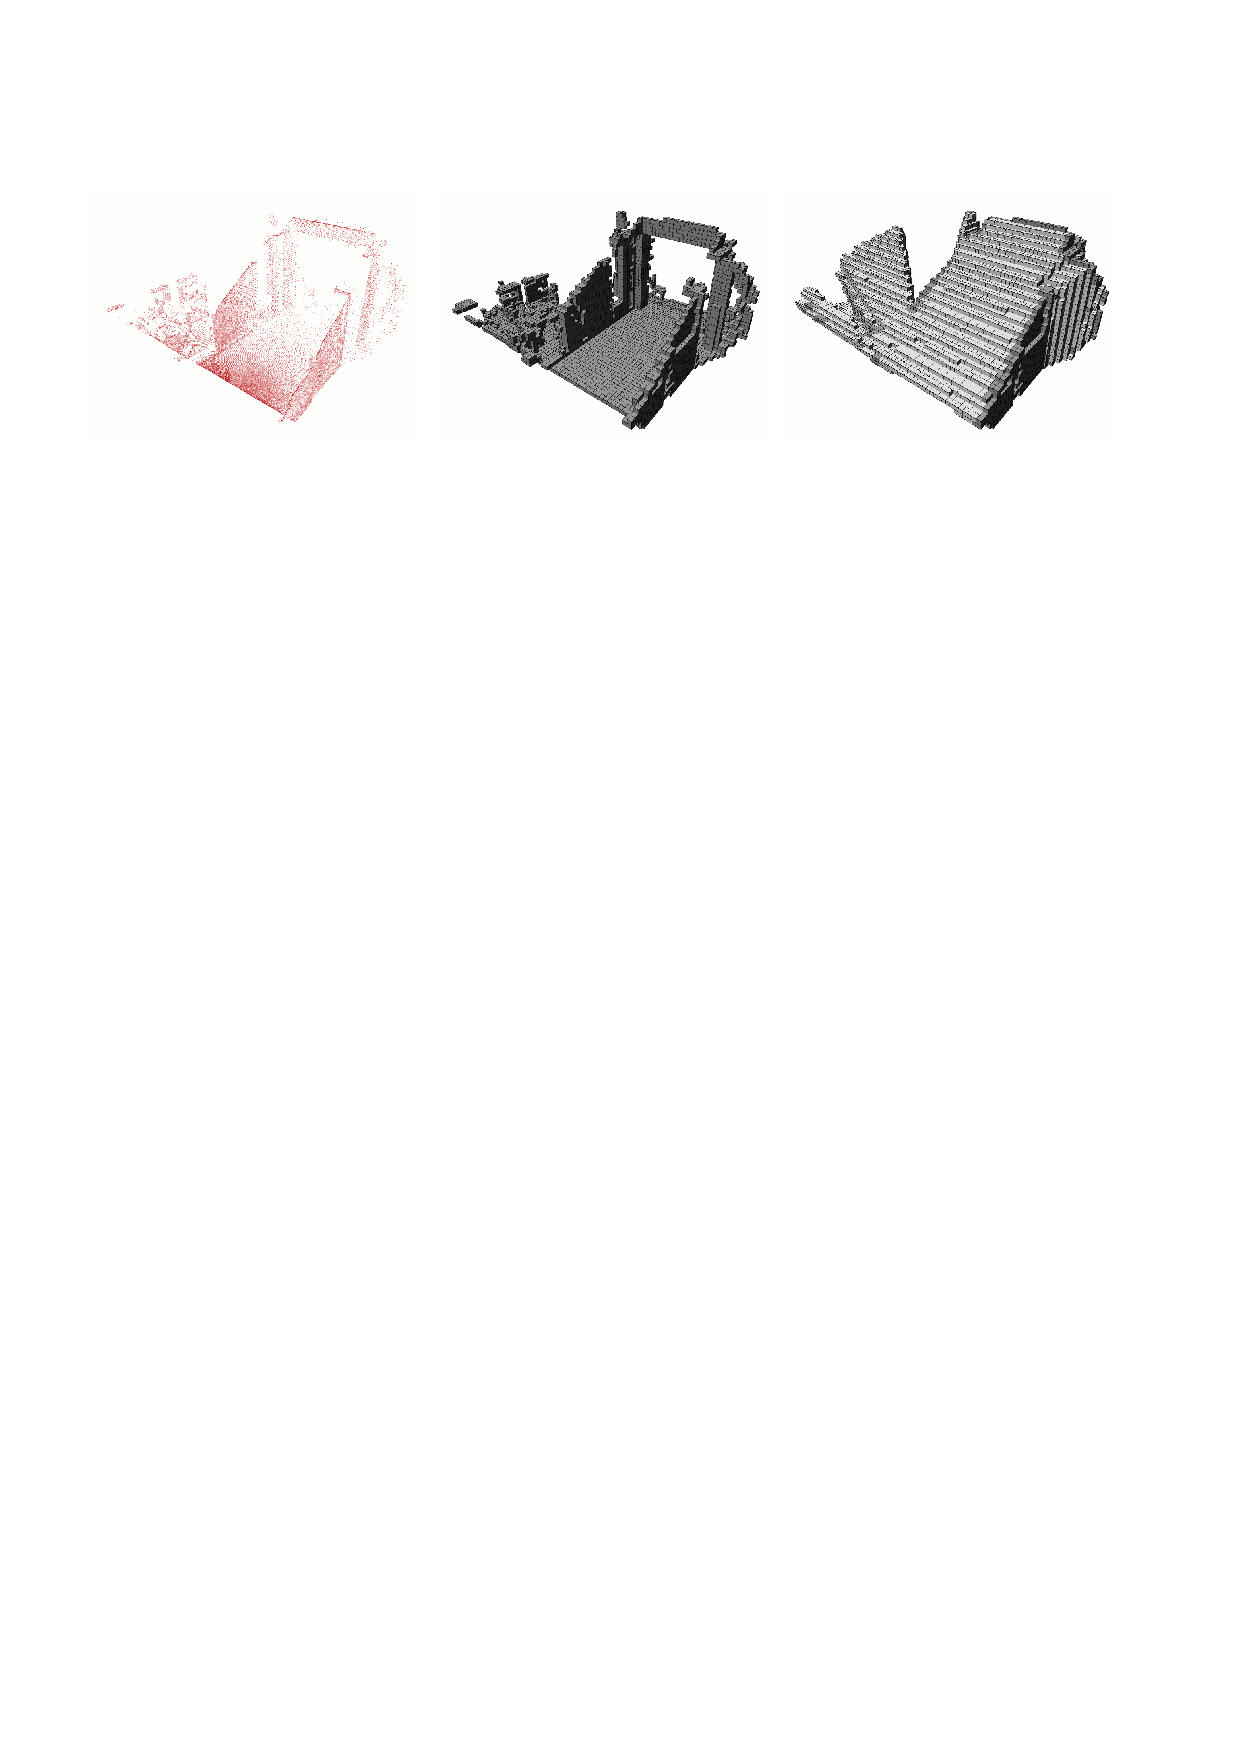
\includegraphics[width=0.95\textwidth]{figs/3d/free}
    \caption{\textit{Esquerda:} Representação do ambiente utilizando pointclouds e sem a possibilidade de se diferenciar espaços desconhecidos e vazios. \textit{Meio:} Representação em octomap com os espaços vazios omitidos. \textit{Direita:} Representação em octomap com os espaços vazios em cinza claros e os ocupados em cinza escuro.}
    \label{fig:free}
\end{figure}
\end{itemize}

\paragraph{Conclusão de análise técnica}\mbox{}\\
A representação 3D do ambiente a ser inspecionado por meio da utilização de Octomap se mostrou, além de mais eficiente no quesito de consumo de memória, perfeitamente alinhada com as necessidades particulares da solução a ser proposta. A possibilidade de busca e segmentação do mapa, possibilita a análise de partes isoladas do mapa e, consequentemente, a identificação de objetos esperados, assim como objetos estranhos e que não deveriam estar presentes. A diferenciação entre espaços vazios e cheios e a política de ocupância probabilística exercem uma função de segurança, a medida que explicitam qual parte do ambiente já foi inspecionada e atenuam possíveis ruídos externos e, também, intrínsecos ao sensor.
